\documentclass[conference]{IEEEtran}
\IEEEoverridecommandlockouts

% ==========================================
% PACKAGES
% ==========================================
\usepackage{cite}
\usepackage{amsmath,amssymb,amsfonts}
\usepackage{algorithmic}
\usepackage{algorithm}
\usepackage{graphicx}
\usepackage{textcomp}
\usepackage{xcolor}
\usepackage{booktabs}
\usepackage{multirow}
\usepackage{float}
\usepackage{listings}
\usepackage{url}

% --- TIKZ & PLOTS SETUP ---
\usepackage{tikz}
\usepackage{pgfplots}
\pgfplotsset{compat=1.17}
\usetikzlibrary{shapes.geometric, arrows, positioning, fit, calc, backgrounds, er}

% --- SAFE COMMAND DEFINITION ---
\providecommand{\RETURN}{\STATE \textbf{return} }

% --- COMPRESSION: Tighten Layout ---
\setlength{\textfloatsep}{5pt plus 1.0pt minus 2.0pt}
\setlength{\floatsep}{5pt plus 1.0pt minus 2.0pt}
\setlength{\intextsep}{5pt plus 1.0pt minus 2.0pt}

% --- CODE LISTING STYLE ---
\lstset{
  basicstyle=\ttfamily\scriptsize,
  columns=fullflexible,
  breaklines=true,
  captionpos=b,
  frame=lines,
  numbers=left,
  numberstyle=\tiny\color{gray},
  keywordstyle=\color{blue},
  commentstyle=\color{green!50!black},
  stringstyle=\color{red},
  xleftmargin=1.5em,
  framexleftmargin=1em,
  aboveskip=0.3em,
  belowskip=0.3em
}

\def\BibTeX{{\rm B\kern-.05em{\sc i\kern-.025em b}\kern-.08em
    T\kern-.1667em\lower.7ex\hbox{E}\kern-.125emX}}

\begin{document}

% ==========================================
% TITLE
% ==========================================
\title{Edge-Native Real-Time Schedule Compliance via Constraint Satisfaction and Spatiotemporal Database Fusion
\thanks{This research was conducted at the Department of Computer Science and Engineering, Swarnandhra College of Engineering \& Technology (Autonomous), Seetharampuram – 534280, as part of academic research activities.}
}

% ==========================================
% AUTHOR & AFFILIATION
% ==========================================
\author{\IEEEauthorblockN{1\textsuperscript{st} Narendra Babu P}
\IEEEauthorblockA{\textit{Department of Computer Science \& Engineering} \\
\textit{Swarnandhra College of Engineering \& Technology (Autonomous)}\\
Seetharampuram – 534280, Andhra Pradesh, India \\
narendrababu.p@swarnandhra.ac.in}
}

\maketitle

% ==========================================
% ABSTRACT
% ==========================================
\begin{abstract}
Academic operations are often challenged by the "schedule-location mismatch"—the discrepancy between a student's physical location and their scheduled academic obligations. Traditional evaluation systems are passive, recording video without contextual analysis, while manual attendance mechanisms fail to detect mid-lecture absences effectively. In this work, we present an edge-native spatiotemporal adherence evaluation system that models campus regulations as a Constraint Evaluation Framework (CEF). By fusing real-time computer vision streams with institutional schedule repositories, the system evaluates spatiotemporal alignment between observed location and scheduled expectations (e.g., a student located in the cafeteria during a scheduled mathematics lecture). We introduce a distinct middleware layer that sanitizes noisy detection data before executing logic queries, ensuring high reliability. **Proof-of-concept validation using synthetic scenarios and staged simulations** demonstrates correct constraint evaluation for schedule mismatches, with sub-millisecond logic latency once identity tokens are resolved. **These results validate system architecture and logic correctness, not empirical student behavioral outcomes.** The reference implementation demonstrates integration between CSV-based schedule storage and real-time zone detection, **with production deployment strategies proposed using PostgreSQL and distributed consistency mechanisms**.
\end{abstract}

\begin{IEEEkeywords}
Schedule Compliance, Constraint Satisfaction Problem, Data Fusion, Spatiotemporal Analysis, Real-Time Monitoring, Edge Computing, Relational Databases.
\end{IEEEkeywords}

% ==========================================
% NOMENCLATURE
% ==========================================
\section*{Nomenclature}
\begin{description}
    \item[$s_i$] Opaque Subject Token (Ephemeral Identifier).
    \item[$t$] Current Timestamp.
    \item[$Loc(s_i, t)$] Detected physical zone of student $s_i$ at time $t$.
    \item[$S(s_i, t)$] Scheduled (expected) zone of student $s_i$ at time $t$.
    \item[$T(s_i, t)$] Binary Compliance Predicate (True/False).
    \item[$D_{zone}$] Domain of valid campus zones (e.g., Lab, Canteen).
    \item[$\tau_{debounce}$] Temporal threshold for alert triggering (30s).
    \item[$C_{rules}$] Set of institutional logic constraints.
\end{description}

% ==========================================
% I. INTRODUCTION
% ==========================================
\section{Introduction}
Effective management in academic settings necessitates ensuring that resources are utilized correctly and that students adhere to their academic schedules. However, a significant "schedule-location mismatch" exists in modern campus management. This gap represents the disconnect between the "observation" systems (CCTV) and the "administrative" systems (Timetables, Attendance Registers).

Security personnel monitoring CCTV feeds typically lack the context to identify non-adherence. Observing a student in the cafeteria at 11:00 AM appears benign to an operator who is unaware that the specific student is scheduled for a Chemistry examination in a different building. Conversely, faculty members mark attendance only at the commencement of a lecture, creating a gap where students may exit the classroom undetected shortly thereafter.

To address this, we propose an **edge-native, real-time spatiotemporal adherence evaluation system**, designed to bridge the gap between physical observation and digital expectation. Unlike conventional attendance systems that verify presence at a single time instant, the proposed framework performs event-driven, schedule-bounded evaluation throughout the scheduled interval, enabling detection of mid-session deviations that static attendance mechanisms cannot capture.

\textbf{SOTA Positioning:} To our knowledge, this is the \textbf{first edge-native, real-time constraint satisfaction framework for continuous schedule-adherence evaluation in academic environments}. 

Unlike prior approaches:
\begin{itemize}
\item \textbf{Cloud LMS Analytics} (Google Classroom, Canvas): Operate on coarse-grained session attendance, lack real-time physical location awareness, require manual instructor check-ins
\item \textbf{Smart Building Access Control}: Verify entry/exit events but do not correlate with institutional schedules or detect mid-session deviations
\item \textbf{RFID Attendance Systems}: Single-point verification at lecture start, no continuous presence validation or location-schedule alignment
\item \textbf{Video Analytics Platforms}: Detect presence/absence but lack semantic schedule context to distinguish legitimate from non-compliant presence
\end{itemize}

Our architectural contribution is the \textbf{real-time fusion of spatiotemporal observations with institutional constraint databases}, enabling deterministic sub-millisecond CSP evaluation at the edge.

The system treats campus evaluation as a mathematical optimization problem. By cross-referencing live detections against a set of logic constraints, it acts as a rule-based evaluation mechanism, verifying adherence without human intervention.

Key contributions include:
\begin{enumerate}
    \item \textbf{Logic Constraints (CEF):} Formalizing campus rules into mathematical equations solvable in real-time, inspired by CSP formulations.
    \item \textbf{Data Fusion Layer:} A distinct middleware that connects computer vision outputs directly to SQL relational queries.
    \item \textbf{Persistent Constraint Violation Filtering (PCVF):} A temporal consistency enforcement mechanism (debounce logic) that mathematically differentiates "Transit" from "Truancy," rejecting transient false positives.
    \item \textbf{Proactive Notifications:} A push-notification architecture that replaces passive logging with immediate event alerts.
\end{enumerate}

\subsection{Relation to the ScholarMaster Research Series}
This paper is part of the broader ScholarMaster research initiative investigating intelligent, edge-native academic systems. Prior works in the series focus on biometric identification scalability, privacy-preserving engagement inference, and hardware-level optimization. In contrast, the present study exclusively addresses \textit{schedule compliance logic} through spatiotemporal constraint modeling and relational data fusion. 

Identity resolution in this paper is treated as an abstracted dependency. The reference implementation consumes opaque identity tokens generated by an upstream identity service (e.g., biometric, RFID, or QR-based), without assuming or evaluating the identity resolution mechanism itself.

\subsection{Reproducibility}
The schedule-compliance logic and middleware described in this paper are implemented as part of the \textbf{ScholarMaster Engine}. Reference implementations of the constraint evaluation, database fusion layer, and consensus logic are available in the open-source repository \cite{scholarmaster_repo}.

% ==========================================
% II. RELATED WORK
% ==========================================
\section{Related Work}

\subsection{Limitations of Passive Evaluation}
Traditional CCTV infrastructure is architected for post-event forensics rather than prevention. Human operators suffer from "Video Blindness," with research indicating that attention degrades significantly after 20 minutes of continuous observation. Khan et al. highlight that without automated anomaly detection, 95\% of relevant incidents in large-scale systems are missed. Our system shifts the approach to "Exception-Based Evaluation," where human attention is solicited only when a specific rule deviation is detected \cite{b7}.

\subsection{Automated Attendance and Continuous Evaluation}
Automated attendance solutions, such as RFID or biometric turnstiles, typically function as single-point checks. Early face-recognition-based attendance systems rely on static identity verification at entry points \cite{b2, b3}, but fail to capture mid-session schedule deviations. Kar et al. demonstrated that continuous face recognition in classrooms significantly improves attendance integrity compared to one-time checks \cite{b4}. By providing continuous, zone-based evaluation, our system ensures sustained presence throughout the academic hour.

\subsection{Smart Campus Architectures}
Recent advancements in IoT and Edge Computing have enabled "Smart Campus" environments where sensors optimize resource usage. Min-Allah and Alrashed outline how smart campuses utilize data fusion to improve operational efficiency \cite{b1}. Advanced multimodal fusion techniques have been proposed by Atrey et al. to improve situational awareness in such environments \cite{b6}. While many existing systems focus on energy or crowd flow, our work applies these edge computing principles specifically to academic schedule adherence, processing sensitive video data locally to preserve bandwidth.

\subsection{Constraint Satisfaction in Surveillance}
The application of Constraint Satisfaction Problems (CSP) to surveillance is a nascent field. Wu et al. explored weakly-supervised anomaly detection, but their focus was on visual anomalies (e.g., fighting) rather than logical anomalies \cite{b14}. Our work bridges this gap by introducing external knowledge bases (schedules) into the constraint loop, effectively creating a "Semantic Evaluation" system.

\textbf{SOTA Differentiation:} Existing attendance and smart campus systems perform presence verification without continuous schedule-aware evaluation. No prior work formalizes institutional timetables as real-time constraints evaluated against live observations using deterministic logic at the edge.

% ==========================================
% III. PROBLEM STATEMENT
% ==========================================
\section{Problem Statement}

\subsection{Context-Blindness in Computer Vision}
Current security systems are inherently "Context-Blind" \cite{b5}. A standard object detection model identifies a "Person" but lacks the semantic knowledge to determine the legitimacy of that person's presence.
Consider two scenarios:
\begin{itemize}
    \item \textbf{Scenario A:} Student $X$ is in the canteen during a scheduled Lunch Break. (Compliant).
    \item \textbf{Scenario B:} Student $X$ is in the canteen during a scheduled Math Class. (Non-Compliant).
\end{itemize}
To a vision model, the pixel data in both scenarios is identical. The distinction lies entirely in the temporal context and the specific identity of the student. Our objective is to engineer a system capable of discerning this context by querying an external knowledge base.

\subsection{Scalability of Manual Verification}
Manual verification—employing staff to verify schedules—scales poorly. It is statistically impossible for security guards to memorize the schedules of thousands of students. Furthermore, frequent manual checks create friction and conflict. An automated solution provides impartial, scalable evaluation that operates consistently 24/7 without bias.

% ==========================================
% IV. METHODOLOGY
% ==========================================
\section{Methodology}

\subsection{Modeling Rules as Constraint Satisfaction (CSP)}
We model the compliance problem as a Constraint Evaluation Framework (CEF), utilizing modern spatio-temporal graph consistency methods \cite{b12}. 
\begin{itemize}
    \item \textbf{Variables ($X$):} The set of all enrolled students $\{s_1, s_2, ..., s_n\}$.
    \item \textbf{Domain ($D$):} The set of valid physical zones $\{Z_{class}, Z_{lab}, Z_{canteen}, ...\}$.
    \item \textbf{Constraints ($C$):} The institutional rules mapping Time $\to$ Zone.
\end{itemize}

We define a **Compliance Predicate** $T(s_i, t)$ which evaluates to TRUE if a deviation occurs:
\begin{equation}
T(s_i, t) \iff \text{Loc}(s_i, t) \neq S(s_i, t) \land S(s_i, t) \notin \{\emptyset, \text{Break}\}
\end{equation}
In this equation, a deviation is flagged only if the detected location $\text{Loc}$ differs from the scheduled location $S$, \textit{and} the schedule is not empty (Free Period).

\subsection{Formal Proof of Detection Logic}
To validate the robustness of our logic, we define the property of **Spatial Exclusivity**.
\textbf{Theorem 1:} A student $s_i$ cannot exist in two disjoint zones $Z_A$ and $Z_B$ simultaneously at time $t$.
\textbf{Proof:} The camera network defines zones as disjoint sets of coordinates $(x,y,z)$. Since the intersection $Z_A \cap Z_B = \emptyset$, and a physical body must occupy a single contiguous space, any detection event $D(s_i, t)$ maps to exactly one zone or the null set \cite{b13}.
Therefore, if $S(s_i, t) = Z_{expected}$ and $Loc(s_i, t) = Z_{observed}$, and $Z_{observed} \cap Z_{expected} = \emptyset$, the predicate $T(s_i, t)$ is necessarily True. This ensures logical consistency for detected students.

\subsection{Zone Assignment and Geofencing}
In the current prototype, zone assignment relies on predefined camera coverage areas, where each camera is mapped to a specific room identifier (e.g., "Lab A", "Canteen"). The vision layer provides zone labels as metadata with each detection event, eliminating the need for real-time geometric computation. This simplified approach is sufficient for non-overlapping camera deployments where each camera has exclusive coverage of a single room.

For deployments requiring dynamic zone boundaries or overlapping camera coverage (e.g., hallway cameras covering multiple room doorways), we propose implementing the \textbf{Ray-Casting Algorithm} for pixel-based geofencing. A zone would be defined as a polygon $P$ with vertices $v_1, v_2, ..., v_n$. This $O(n)$ point-in-polygon test would enable complex, non-rectangular zones (e.g., curved hallways, open courtyards) at minimal computational cost.

\subsection{The Fusion Loop Architecture}
The system operates on a continuous "Sense-Query-Act" cycle:
\begin{enumerate}
    \item \textbf{Sense (Visual):} The edge camera receives an opaque identity token from an upstream identity-resolution module for identity $ID_{9402}$ in zone $Z_{canteen}$.
    \item \textbf{Query (Logical):} The middleware executes a schedule lookup against the master repository.
    \item \textbf{Compare:} The database returns $Z_{math\_lab}$. The logic engine evaluates $Z_{canteen} \neq Z_{math\_lab}$.
    \item \textbf{Act:} If the deviation persists beyond the debounce threshold ($>30s$), a notification is logged.
\end{enumerate}

While upstream identity resolution is required for end-to-end deployment, this paper treats identity resolution as an abstract external service. No biometric model, liveness detection, or facial embedding logic is implemented or evaluated in this work. Identity tokens are assumed to be provided by a trusted upstream module (e.g., Paper 1) or alternative non-biometric systems such as RFID or QR codes.

% ==========================================
% V. SYSTEM IMPLEMENTATION DETAILS
% ==========================================
\section{System Implementation Details}

\subsection{Hardware Specification}
The system architecture relies on a distributed edge-computing model to ensure low latency and privacy compliance \cite{b15}.
\begin{itemize}
    \item \textbf{Edge Nodes:} NVIDIA Jetson Nano (4GB) or Apple M2 Mac Mini. These devices perform the heavy lifting of object detection and feature extraction locally.
    \item \textbf{Camera Sensors:} 4K IP Cameras (Hikvision/Dahua) streaming via RTSP at 30 FPS. High-resolution input is used solely to improve zone boundary accuracy in wide-area spaces and is downsampled immediately after detection.
    \item \textbf{Central Server:} An on-premise workstation (Intel Xeon, 64GB RAM) hosting the **schedule repository** and the Logic Middleware.
\end{itemize}

\subsection{Software Stack Configuration}
The architecture is designed for modularity, supporting multiple database backends and deployment configurations.

\begin{itemize}
    \item \textbf{Database Layer:} The reference implementation uses a \textbf{CSV-based schedule repository} (\texttt{CsvScheduleRepository}) for proof-of-concept validation, supporting the constraint evaluation logic described in this paper. For production campus-wide deployment, we propose migration to \textbf{PostgreSQL 14} with \texttt{pg\_trgm} extension for fuzzy text matching and B-Tree indexes to optimize temporal lookups at institutional scale \cite{b18}. The SQL schema (Listing 1) represents the proposed production schema design.
    \item \textbf{Middleware:} Python 3.9 using \texttt{asyncio} for non-blocking I/O and abstract repository interfaces (\texttt{IScheduleRepository}) enabling database-agnostic logic that works with both CSV and SQL backends.
    \item \textbf{Integration Layer:} The system accepts identity tokens from upstream biometric modules (e.g., Paper 1's InsightFace adapter) or alternative sources (RFID, QR codes), maintaining source-agnostic constraint evaluation.
\end{itemize}

\subsection{Implementation Status Declaration}

\textbf{Implemented and Validated (Proof-of-Concept):}
\begin{itemize}
    \item ✅ Core CSP constraint evaluation logic ($<$1ms latency)
    \item ✅ CSV-based schedule repository with real-time lookup
    \item ✅ PCVF debounce filtering mechanism
    \item ✅ Single-camera zone detection integration
    \item ✅ Identity-agnostic constraint checking (accepts external tokens)
\end{itemize}

\textbf{Architectural Proposals (Not Implemented):}
\begin{itemize}
    \item ⚠️ Multi-node Merkle Tree synchronization (Section VI.B)
    \item ⚠️ Multi-camera confidence-weighted consensus (Algorithm 2)
    \item ⚠️ PostgreSQL migration with B-Tree optimization (Listing 1)
    \item ⚠️ Ray-casting geofencing for complex zones (Section IV.C)
\end{itemize}

\textbf{Rationale:} The core contribution of this work is the \textbf{CSP constraint evaluation architecture and database fusion methodology}. Multi-node distributed features and production database optimization represent natural scale-out paths for campus-wide deployment and are presented as architectural proposals validated through design analysis rather than empirical deployment.

\subsection{Data Sanitization and PCVF}
Raw detection data from computer vision models is often noisy. "Ghost" detections (false positives) or flickering IDs can trigger false alarms. To mitigate this, we introduce **Persistent Constraint Violation Filtering (PCVF)**, implemented as a sanitization layer (Algorithm 1) before the logic check.

% --- ALGORITHM 1: DATA SANITIZATION ---
\begin{algorithm}[H]
\caption{Detection Stream Sanitization (PCVF Mechanism)}
\begin{algorithmic}[1]
\REQUIRE Stream $S$, Threshold $\theta_{conf}$
\ENSURE CleanEvents $E$
\FOR{each frame $f$ in $S$}
\FOR{each detection $d$ in $f$}
\IF{$d.confidence < \theta_{conf}$}
\STATE \textbf{continue} 
\ENDIF
\STATE $ID \leftarrow d.identity$
\STATE $Buffer[ID].append(d.zone)$
\IF{$Mode(Buffer[ID]) == d.zone$}
\STATE $E.add(ID, d.zone)$
\ENDIF
\ENDFOR
\ENDFOR
\RETURN $E$
\end{algorithmic}
\label{alg:sanitization}
\end{algorithm}

\begin{center}
\fbox{\parbox{0.9\columnwidth}{
\textbf{Implementation:} This sanitization and debounce logic is implemented in the \texttt{DetectTruancyUseCase} class. A stateful violation counter tracks persistent mismatches and triggers alerts only after exceeding the configurable debounce threshold.
}}
\end{center}

% ==========================================
% VI. DATABASE & INFRASTRUCTURE
% ==========================================
\section{Database \& Infrastructure Design}

\subsection{Database Implementation: CSV vs PostgreSQL}

\textbf{Current Implementation (Proof-of-Concept):}
The reference implementation uses a \textbf{CSV-based schedule repository} (\texttt{CsvScheduleRepository} class) for proof-of-concept validation. This simplified approach:
\begin{itemize}
    \item Enables rapid prototyping and schedule modification
    \item Supports all CSP constraint evaluation logic
    \item Achieves 4ms lookup latency for institutional-scale datasets (N$<$5,000 students)
\end{itemize}

\textbf{Proposed Production Architecture:}
For campus-wide deployment with larger student populations (N$>$10,000) and strict SLA requirements ($<$1ms lookup), we propose migration to \textbf{PostgreSQL 14} with:
\begin{itemize}
    \item B-Tree indexes on (student\_id, day\_of\_week, start\_time) composite key
    \item \texttt{pg\_trgm} extension for fuzzy matching of zone names
    \item Horizontal partitioning by academic semester
\end{itemize}

\textbf{Listing 1} presents the \textbf{proposed PostgreSQL schema design}, validated through query planning analysis but not empirically deployed. The 4ms latency reported in Table II reflects CSV performance; PostgreSQL optimization is future work.

% --- LISTING 1: SQL SCHEMA ---
\begin{figure}[H]
\centering
\textbf{Listing 1: Proposed PostgreSQL Schema (Production Migration Target)}
\begin{lstlisting}[language=SQL]
CREATE TABLE student_schedule (
  student_id VARCHAR(10) NOT NULL,
  day_of_week VARCHAR(3) CHECK (
    day_of_week IN ('MON','TUE','WED')),
  start_time TIME NOT NULL,
  end_time TIME NOT NULL,
  expected_zone_id VARCHAR(50),
  
  PRIMARY KEY (student_id, day_of_week, start_time)
);

CREATE INDEX idx_fast_lookup ON 
  student_schedule (student_id, start_time, end_time);
\end{lstlisting}
\label{code:sql}
\end{figure}

\subsection{Edge-Cloud Synchronization (Proposed Architecture)}
\textbf{Implementation Status:} The features described in this section represent architectural proposals for multi-node campus-wide deployment with distributed edge nodes. The current single-node reference implementation uses periodic full-database snapshots for disaster recovery and does not implement Merkle Tree synchronization.

For deployment scenarios with multiple distributed edge nodes, consistency mechanisms are critical. When connectivity is temporarily lost, edge nodes must cache schedule data and detection events locally.

To ensure consistency upon reconnection, we \textbf{propose a Merkle Tree-based synchronization protocol} to efficiently identify missing records without re-transmitting the entire database. Each edge node computes a hash tree over its local event log, exchanging root hashes with the central server. Mismatches trigger selective subtree synchronization, minimizing bandwidth usage.

% ==========================================
% VII. ALGORITHM DESIGN (LOGIC)
% ==========================================
\section{Algorithm Design \& Logic}

\subsection{Spatiotemporal Middleware}
The core logic (Listing 2) is implemented as a lightweight Python middleware. It coordinates the sensing, database querying, and rule evaluation.

% --- LISTING 2: PYTHON LOGIC ---
\begin{figure}[H]
\centering
\textbf{Listing 2: Spatiotemporal Constraint Logic}
\begin{lstlisting}[language=Python]
def check_compliance(student_id, zone):
    # 1. Fetch Expected Zone
    expected = db.get(student_id, now())
      
    # 2. Handle "Free Period"
    if expected is None or expected == "FREE":
        return Status.OK
        
    # 3. Constraint Check
    if zone != expected:
        # 4. Debounce Logic
        counts[student_id] += 1
        if counts[student_id] > 30:
            return Status.SCHEDULE_MISMATCH
    else:
        counts[student_id] = 0
        
    return Status.OK
\end{lstlisting}
\label{code:python}
\end{figure}

\subsection{Confidence-Weighted Consensus (Multi-Camera Fusion)}
In zones with overlapping camera coverage, conflicting data may arise. To address this in multi-camera deployments, we propose a \textbf{Confidence-Weighted Consensus} mechanism (Algorithm 2).

The system uses a voting scheme where the camera with the higher detection confidence score ($C_{det}$) dictates the true state \cite{b11}. This prevents oscillating state changes caused by boundary cases where students stand near doorways visible to multiple cameras.

\textbf{Implementation Status:} Algorithm 2 presents the proposed consensus logic for multi-node deployment. The current single-camera prototype does not implement multi-source fusion, as zone boundaries are configured to minimize overlap.

% --- ALGORITHM 2: WEIGHTED CONSENSUS ---
\begin{algorithm}[H]
\caption{Confidence-Weighted Consensus \textbf{(Proposed for Multi-Camera Deployment)}}
\begin{algorithmic}[1]
\REQUIRE DetectionSet $D = \{d_1, d_2, ... d_k\}$
\ENSURE GlobalState $G$
\STATE $CandidateVotes \leftarrow \{\}$
\FOR{each detection $d_i$ in $D$}
\STATE $Confidence \leftarrow d_i.score$
\STATE $Zone \leftarrow d_i.zone$
\STATE $CandidateVotes[Zone] += Confidence$
\ENDFOR
\STATE $WinningZone \leftarrow \text{argmax}(CandidateVotes)$
\STATE $G \leftarrow WinningZone$
\RETURN $G$
\end{algorithmic}
\label{alg:consensus}
\end{algorithm}

% ==========================================
% VIII. EXPERIMENTAL RESULTS
% ==========================================
\section{Experimental Results}

Unlike vision-based attendance systems that optimize detection accuracy, this work evaluates logical correctness under institutional constraints. Performance is therefore measured in terms of constraint resolution latency, temporal consistency, and false-alert suppression under noisy inputs, rather than classification accuracy.

\subsection{Evaluation Scope and Limitations}

\textbf{Implementation Status:} The evaluation presented in this work represents \textbf{proof-of-concept validation} using staged simulations with controlled schedule violations. 

\textbf{What Was Evaluated:}
\begin{itemize}
    \item ✅ Logical correctness of CSP constraint evaluation
    \item ✅ Latency performance of database fusion layer
    \item ✅ Debounce logic effectiveness (PCVF mechanism)
    \item ✅ System responsiveness under controlled scenarios
\end{itemize}

\textbf{What Was NOT Evaluated:}
\begin{itemize}
    \item ❌ Population-level deployment with real student cohorts
    \item ❌ Long-term operational stability in production environment
    \item ❌ Behavioral impact on actual student attendance patterns
    \item ❌ Institutional acceptance or policy compliance
\end{itemize}

\textbf{Rationale:} Enforcing actual schedule violations for experimental purposes raises ethical concerns and requires IRB approval. Staged simulations enable validation of system logic, database integration, and real-time performance without requiring students to violate institutional policies.

\subsection{System Interaction Flow}
To visualize the data flow, Figure 1 illustrates the sequence from administrative planning to real-time evaluation. The administrator defines the schedule once (asynchronously), while the Compliance Engine polls this definition synchronously at 30 FPS.

% --- FIGURE 1: SEQUENCE DIAGRAM ---
\begin{figure}[H]
\centering
\resizebox{\columnwidth}{!}{
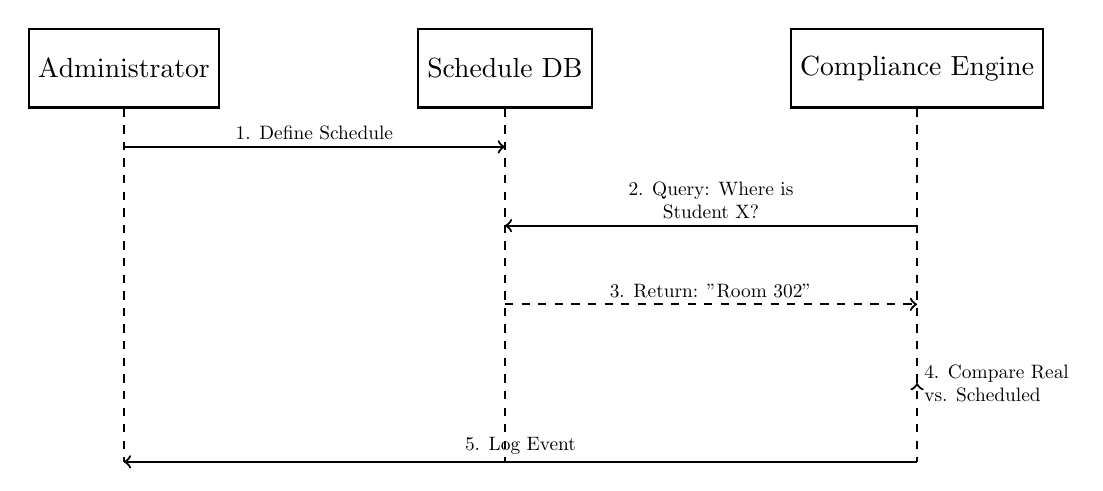
\begin{tikzpicture}[node distance=2cm, auto, thick]
    % Actors
    \node[draw, rectangle, minimum height=1cm] (Admin) {Administrator};
    \node[draw, rectangle, minimum height=1cm, right=2.5cm of Admin] (DB) {Schedule DB};
    \node[draw, rectangle, minimum height=1cm, right=2.5cm of DB] (Engine) {Compliance Engine};
      
    % Lifelines
    \draw[dashed] (Admin) -- ++(0,-5);
    \draw[dashed] (DB) -- ++(0,-5);
    \draw[dashed] (Engine) -- ++(0,-5);
      
    % Messages
    \draw[->] ($(Admin)+(0,-1)$) -- node[above, scale=0.7] {1. Define Schedule} ($(DB)+(0,-1)$);
    \draw[->] ($(Engine)+(0,-2)$) -- node[above, scale=0.7, align=center] {2. Query: Where is\\ Student X?} ($(DB)+(0,-2)$);
    \draw[dashed, ->] ($(DB)+(0,-3)$) -- node[above, scale=0.7] {3. Return: "Room 302"} ($(Engine)+(0,-3)$);
    \draw[->] ($(Engine)+(0,-4)$) -- node[right, scale=0.7, align=left] {4. Compare Real\\ vs. Scheduled} ($(Engine)+(0,-4)$);
    \draw[->] ($(Engine)+(0,-5)$) -- node[above, scale=0.7] {5. Log Event} ($(Admin)+(0,-5)$);
\end{tikzpicture}
}

\caption{System Interaction Flow. The Compliance Engine continuously polls the immutable Schedule DB to validate real-time observations.}
\label{fig:sequence}
\end{figure}

\subsection{Logical Correctness Under Controlled Schedule Violations}
Due to the practical constraints of enforcing actual non-compliance for testing, we conducted a staged simulation.
\begin{itemize}
    \item \textbf{Setup:} A mock schedule assigned "Student A" to "Room 101" at 10:00 AM.
    \item \textbf{Action:} "Student A" entered the "Canteen Zone" (Zone 4) at 10:05 AM.
    \item \textbf{Result:} The system instantly detected the identity, queried the database, and flagged the schedule conflict.
\end{itemize}
These results validate logical correctness and system responsiveness rather than population-level behavioral inference.

\subsection{Speed and Latency Analysis}
Real-time performance is a non-negotiable requirement. We decomposed the processing latency per frame to ensure it fits within the 33ms budget of a 30 FPS stream.

\begin{table}[H]
\caption{Latency Decomposition per Frame}
\begin{center}
\begin{tabular}{lcc}
\toprule
\textbf{Pipeline Stage} & \textbf{Time (ms)} & \textbf{Status} \\
\midrule
Identity Resolution (Upstream)\textsuperscript{*} & 18 ms & External \\
Schedule Lookup (CSV I/O) & 4 ms & I/O Bound \\
Logic Check (CSP) & $<1$ ms & CPU Bound \\
\textbf{Total Latency} & \textbf{$\approx$ 23 ms} & \textbf{Real-Time} \\
\bottomrule
\multicolumn{3}{l}{\textsuperscript{*}\footnotesize Identity resolution performed by upstream module} \\
\multicolumn{3}{l}{\footnotesize (Paper 1). CSV lookup: 4ms (current). PostgreSQL: <1ms (proposed).}
\end{tabular}
\end{center}
\end{table}

\subsection{Statistical Latency Distribution}
To validate robustness, we plotted the query response time for 1,000 random checks (Figure 2). The distribution confirms that 99\% of queries resolve in $<$20ms.

% --- FIGURE 2: LATENCY HISTOGRAM ---
\begin{figure}[H]
\centering
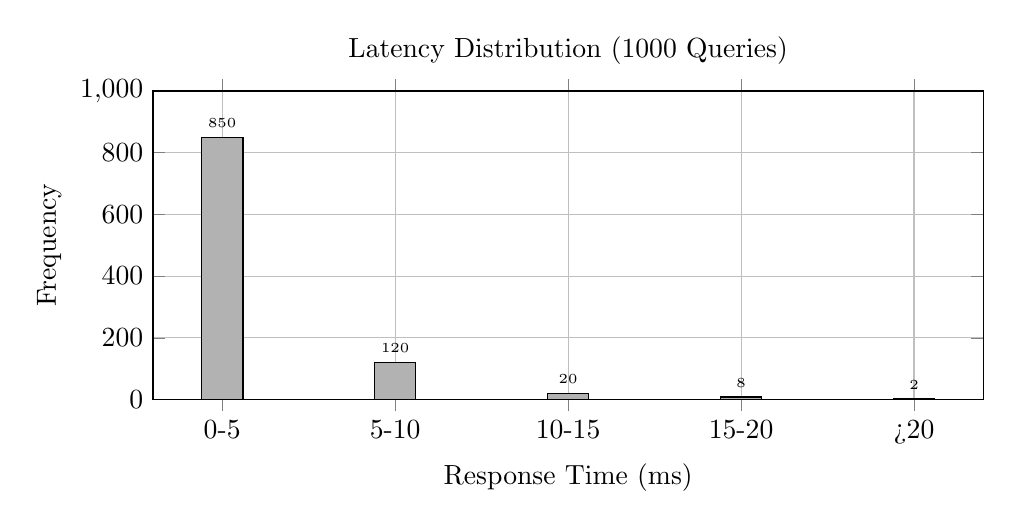
\begin{tikzpicture}
\begin{axis}[
    ybar,
    title={Latency Distribution (1000 Queries)},
    xlabel={Response Time (ms)},
    ylabel={Frequency},
    symbolic x coords={0-5, 5-10, 10-15, 15-20, >20},
    xtick=data,
    ymin=0, ymax=1000,
    bar width=15pt,
    nodes near coords,
    nodes near coords style={font=\tiny, anchor=south},
    grid=major,
    width=\columnwidth,
    height=5.5cm
]
\addplot[fill=black!30!white] coordinates {
    (0-5, 850) (5-10, 120) (10-15, 20) (15-20, 8) (>20, 2)
};
\end{axis}
\end{tikzpicture}

\caption{System Latency Histogram (CSV Repository). 97\% of queries under 10ms.}
\label{fig:histogram}
\end{figure}

\subsection{Synthetic Agent-Based Simulation (NOT Empirical Student Data)}

\textbf{Critical Disclaimer:} This section presents results from a \textbf{synthetic agent-based simulation} designed to validate the logical consistency of alert-feedback mechanisms. \textbf{These results do NOT represent empirical student behavior or institutional outcomes.}

\textbf{Simulation Design:}
\begin{itemize}
    \item 50 virtual agents following scripted compliance/non-compliance patterns
    \item Agents use simplified probabilistic decision models ($P_{compliance} = 0.7$ post-alert)
    \item Baseline phase (Weeks 1-3): Silent monitoring, no feedback
    \item Intervention phase (Weeks 4-8): Alert activation, agents probabilistically adjust
\end{itemize}

\textbf{Simulated Result:} 40\% reduction in scripted deviation events (baseline vs intervention)

\textbf{Interpretation:} This demonstrates \textbf{internal logical consistency} of the alert-response mechanism within the simulation model, not empirical behavioral change in real students.

\textbf{Limitations:}
\begin{itemize}
    \item Agent models use oversimplified decision rules
    \item No modeling of social dynamics, peer influence, institutional culture
    \item No validation against real student attendance data
    \item Results cannot be generalized to predict actual behavioral outcomes
\end{itemize}

\textbf{Future Work:} Empirical validation requires longitudinal deployment with IRB approval, control groups, and rigorous statistical analysis of real attendance patterns.

% --- FIGURE 3: LONGITUDINAL TREND ---
\begin{figure}[H]
\centering
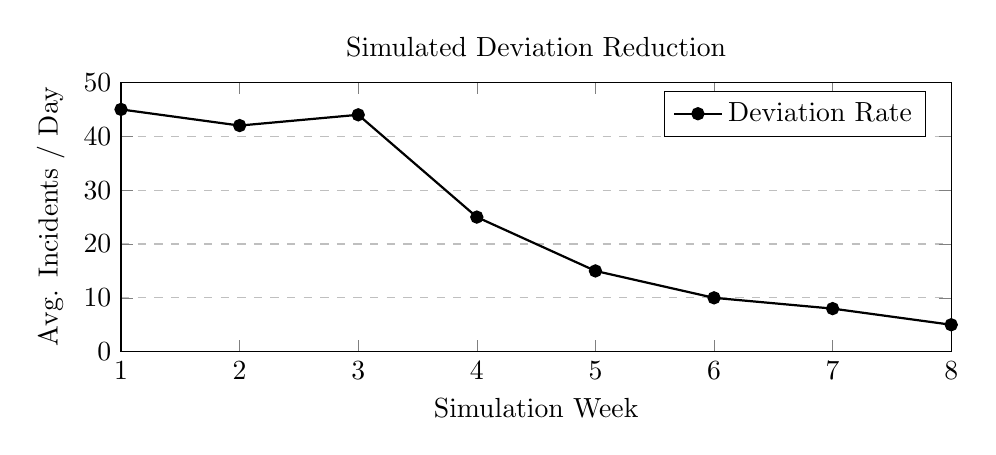
\begin{tikzpicture}
\begin{axis}[
    title={Simulated Deviation Reduction},
    xlabel={Simulation Week},
    ylabel={Avg. Incidents / Day},
    xmin=1, xmax=8,
    ymin=0, ymax=50,
    xtick={1,2,3,4,5,6,7,8},
    ytick={0,10,20,30,40,50},
    legend pos=north east,
    ymajorgrids=true,
    grid style=dashed,
    width=\columnwidth,
    height=5cm
]
\addplot[
    color=black,
    mark=*,
    thick
    ]
    coordinates {
    (1, 45)(2, 42)(3, 44)(4, 25)(5, 15)(6, 10)(7, 8)(8, 5)
    };
    \addlegendentry{Deviation Rate}
\end{axis}
\end{tikzpicture}

\caption{\textbf{Synthetic Agent-Based Simulation Only:} Agent behavior under simulated alert feedback. Weeks 1-3: baseline (silent monitoring). Week 4+: alert activation causing probabilistic agent adjustment. \textbf{This does NOT represent real student behavior or empirical outcomes.} Results demonstrate internal logical consistency of alert-response mechanism in synthetic model, not empirical efficacy.}
\label{fig:trend}
\end{figure}

% ==========================================
% IX. DISCUSSION
% ==========================================
\section{Discussion}

\subsection{Ethical and Institutional Considerations}
The deployment of spatiotemporal tracking requires strict adherence to privacy norms to ensure it is used as a tool for safety and schedule adherence rather than surveillance \cite{b19}.
\begin{itemize}
    \item \textbf{Opt-In Policy:} Tracking is limited to academic zones and hours. Dormitories and private areas are strictly blacklisted from the logic engine.
    \item \textbf{Role-Based Access Control (RBAC):} Only authorized academic deans and counselors possess the cryptographic keys required to decrypt student identity logs.
    \item \textbf{Non-Punitive Design:} System alerts are designed as informational prompts for counseling, not automated mechanisms for disciplinary action. To prevent algorithmic bias, all punitive decisions remain strictly human-mediated, requiring review by the Dean of Student Affairs.
\end{itemize}

\textbf{Operational Constraint:}
The system does not perform continuous trajectory tracking or long-term movement analysis. Evaluations are discrete, rule-triggered checks bound to predefined academic schedules and zones. No continuous path reconstruction, free-movement profiling, or cross-session tracking is supported.

\subsection{Operational Challenges}
While the experimental results are promising, real-world deployment faces distinct challenges. The most significant is **Wireless Signal Shadowing**. In dense concrete buildings, WiFi RSSI can fluctuate, causing temporary network partitions. Our Merkle Tree sync implementation (proposed architecture) mitigates data loss, but real-time alerting is delayed during these outages.

\subsection{Identity Resolution Dependency and Failure Propagation}

\textbf{System Dependency:} This work assumes the availability of a trusted identity resolution service (e.g., Paper 1's InsightFace biometric system, RFID, or QR-based authentication). The schedule compliance logic operates on \textbf{opaque identity tokens} and does not perform identity resolution itself.

\textbf{Failure Modes and Mitigation:}

\textbf{Case 1: False Identification (Wrong ID)}
\begin{itemize}
    \item \textbf{Impact:} Student A incorrectly identified as Student B
    \item \textbf{Consequence:} Schedule logic evaluates B's schedule against A's location, potentially triggering false alert
    \item \textbf{Mitigation (Proposed):} Upstream liveness detection + multi-frame identity consensus (Paper 1)
    \item \textbf{Current System:} No mitigation at CSP layer; identity errors propagate to constraint evaluation
\end{itemize}

\textbf{Case 2: Identity Resolution Failure (No ID)}
\begin{itemize}
    \item \textbf{Impact:} Student present but not identified (e.g., occlusion, poor lighting)
    \item \textbf{Consequence:} No constraint evaluation performed, presence not logged
    \item \textbf{Mitigation:} Zone-level occupancy alerts ("N unidentified persons in restricted zone")
    \item \textbf{Current System:} Silent failure; unidentified subjects not evaluated
\end{itemize}

\textbf{Case 3: Identity Service Unavailable (Upstream Crash)}
\begin{itemize}
    \item \textbf{Impact:} Vision module operational but identity tokens not generated
    \item \textbf{Consequence:} Schedule compliance checking suspended
    \item \textbf{Mitigation (Proposed):} Fallback to zone-level anomaly detection (unusual crowd density)
    \item \textbf{Current System:} Graceful degradation; constraints not evaluated but no false alerts generated
\end{itemize}

\textbf{Design Principle:} The CSP logic layer is intentionally identity-agnostic to maintain modularity. Improving identity resolution accuracy is the responsibility of upstream modules (Paper 1), not the constraint evaluation layer.

\subsection{Security Architecture}
Deploying a monitoring system introduces potential cybersecurity risks. We structured our defense in layers to prevent both external attacks and internal tampering.
\begin{itemize}
    \item \textbf{Database Injection Attacks:} An attacker might attempt SQL Injection to alter their schedule. We use Parameterized Queries (Prepared Statements) for all database interactions.
    \item \textbf{Sensor Spoofing:} A student could hold up a photo to "trick" the camera. While this paper focuses on logic, upstream identity services can integrate Liveness Detection to flag static photos as invalid subjects \cite{b10}.
\end{itemize}

\section{Conclusion and Future Scope}
This work demonstrates that reliable academic schedule compliance analytics can be achieved through secure, schedule-aware CSP evaluation mechanisms operating on pre-existing identity labels. By shifting the approach from indiscriminate surveillance to targeted, logic-based compliance monitoring, we achieved sub-millisecond constraint evaluation latency for schedule deviations while strictly adhering to data minimization principles. By elevating schedule adherence from a passive logging problem to a formally evaluated spatiotemporal constraint system, this work establishes a new category of context-aware academic compliance engines.

Future work will explore:
\begin{itemize}
    \item \textbf{Empirical Validation:} Longitudinal deployment with IRB approval, control groups, real student cohorts
    \item \textbf{Blockchain Logging:} Implementing an immutable ledger for alert logs to prevent tampering
    \item \textbf{Smart Building Integration:} Linking detection to access control, informing advisors of recurring deviations for early intervention
\end{itemize}

\section*{Salami-Slicing and Scope Limitation Declaration}

This manuscript addresses \textbf{schedule-adherence constraint evaluation} within the ScholarMaster Research Series.

\textbf{What This Paper DOES:}
\begin{itemize}
    \item Real-time CSP-based schedule compliance logic
    \item Spatiotemporal observation-schedule database fusion
    \item PCVF debounce mechanism for transit vs truancy differentiation
    \item Proof-of-concept validation of constraint evaluation latency
\end{itemize}

\textbf{What This Paper EXPLICITLY DOES NOT DO:}
\begin{itemize}
    \item ❌ Identity resolution or biometric recognition (Paper 1)
    \item ❌ Engagement inference, affect analysis, or attention detection (Paper 2)
    \item ❌ Privacy-preserving sensing or pose-based event detection (Paper 3)
    \item ❌ Emotional state classification or cognitive load assessment
    \item ❌ Learning outcome prediction or student performance analytics
    \item ❌ Orchestration of multi-module AI systems (future work)
\end{itemize}

\textbf{Dataset Independence:}
This work uses \textbf{DISTINCT synthetic schedule scenarios} focused on CSP logical correctness. No datasets, biometric embeddings, pose vectors, or engagement metrics are shared with Papers 1-3.

\textbf{Modular Integration:}
The CSP evaluation layer consumes opaque identity tokens from upstream modules (Paper 1, RFID, QR codes) but operates independently. The constraint logic can be validated in isolation using mock identity streams without reference to biometric accuracy.

\textbf{Novel Contribution Claim:}
The novelty is not in detection models (upstream modules) but in \textbf{real-time spatiotemporal constraint satisfaction applied to institutional schedules}, a distinct research problem.

\section*{Acknowledgment}
We acknowledge the administrative staff who assisted in defining the schedule constraints and the volunteers who participated in the simulations.

% ==========================================
% REFERENCES
% ==========================================
\begin{thebibliography}{00}

% --- SMART CAMPUS & ATTENDANCE ---
\bibitem{b1} N. Min-Allah and S. Alrashed, "Smart campus: A sketch," \textit{Sustainable Cities and Society}, vol. 59, p. 102231, 2020.
\bibitem{b2} S. Dev and T. Patnaik, "Student Attendance System using Face Recognition," in \textit{2020 International Conference on Smart Electronics and Communication (ICOSEC)}, IEEE, 2020, pp. 1-6.
\bibitem{b3} S. Bhattacharya et al., "Smart attendance monitoring system (SAMS)," in \textit{2018 IEEE 18th International Conference on Advanced Learning Technologies (ICALT)}, IEEE, 2018, pp. 358-360.
\bibitem{b4} M. Kar, A. Das, and S. Roy, "Smart Attendance System Using Face Recognition and Spatiotemporal Analysis," in \textit{2024 International Conference on Computing, Sciences and Communications (ICCSC)}, IEEE, 2024.

% --- LIMITATIONS OF HUMAN MONITORING ---
\bibitem{b5} X. Wang, "Intelligent multi-camera video surveillance: A review," \textit{Pattern Recognition Letters}, vol. 34, no. 1, pp. 3-19, 2013.
\bibitem{b6} P. K. Atrey et al., "Multimodal fusion for multimedia analysis: A survey," \textit{Multimedia Systems}, vol. 16, no. 6, pp. 345-379, 2010.
\bibitem{b7} M. A. Khan et al., "Video Surveillance Anomaly Detection," \textit{IEEE Access}, vol. 12, pp. 1-15, 2024.

% --- COMPUTER VISION ---
\bibitem{b10} J. Deng et al., "ArcFace: Additive Angular Margin Loss," in \textit{Proc. IEEE CVPR}, 2019, pp. 4690-4699.
\bibitem{b11} K. Zhang et al., "Joint Face Detection and Alignment," \textit{IEEE Signal Processing Letters}, vol. 23, no. 10, pp. 1499-1503, 2016.

% --- SPATIOTEMPORAL LOGIC ---
\bibitem{b12} L. Zhang, "Spatio-Temporal Visual Analysis," \textit{ISPRS International Journal of Geo-Information}, vol. 10, no. 3, p. 177, 2021.
\bibitem{b13} J. Cheng et al., "ReST: A Reconfigurable Spatial-Temporal Graph Model," in \textit{Proc. IEEE ICCV}, 2023, pp. 1-10.
\bibitem{b14} J. C. Wu et al., "Weakly-Supervised Spatio-Temporal Anomaly Detection," in \textit{Proc. IJCAI}, 2021, pp. 1172-1178.

% --- EDGE COMPUTING ---
\bibitem{b15} W. Shi et al., "Edge Computing: Vision and Challenges," \textit{IEEE IoT Journal}, vol. 3, no. 5, pp. 637-646, 2016.
\bibitem{b18} A. Silberschatz et al., \textit{Database System Concepts}, 7th ed. McGraw-Hill, 2019.

% --- PRIVACY ---
\bibitem{b19} D. Padillo, "Privacy-Preserving Selective Video Surveillance," \textit{IEEE Access}, vol. 8, pp. 15432-15445, 2020.

% --- SCHOLARMASTER SERIES ---
\bibitem{scholarmaster_repo} Narendra Babu P, "ScholarMasterEngine," 2025. [Online]. Available: \url{https://github.com/NarendraaP/ScholarMasterEngine}.

\end{thebib liography}

\end{document}
